\begin{frame}{$\Flow$ формулы}
    \begin{minipage}{0.5 \linewidth}
        \tikzstyle{undir} = [thick]
\tikzstyle{dir} = [thick, ->, bend left = 10]
\tikzstyle{ver} = [thick, ->, draw, circle]

\begin{tikzpicture}[black, >=latex]
    \node[ver] (A) at (0, 0) {};
    \node[ver] (B) at (1.9, 1.9) {};
    \node[ver] (C) at (3, 0) {};
    \node[ver] (D) at (4, 1.2) {};
    \node[ver] (E) at (3.3, 3.7) {};
    \node[ver] (F) at (-0.5, 3) {};
    \node at (0, -0.2) {};

    \only<1>{
        \draw[undir] (A) to (B);
        \draw[undir] (A) to (C);
        \draw[undir] (B) to (C);
        \draw[undir] (C) to (D);
        \draw[undir] (B) to (D);
        \draw[undir] (D) to (E);
        \draw[undir] (E) to (F);
        \draw[undir] (F) to (A);
        \draw[undir] (B) to (F);
    }
    
	\only<2->{
        \draw[dir] (A) to (B);
        \draw[dir] (A) to (C);
        \draw[dir] (B) to (C);
        \draw[dir] (C) to (D);
        \draw[dir] (B) to (D);
        \draw[dir] (D) to (E);
        \draw[dir] (E) to (F);
        \draw[dir] (F) to (A);
        \draw[dir] (B) to (F);

        \draw[dir] (B) to (A);
        \draw[dir] (C) to (A);
        \draw[dir] (C) to (B);
        \draw[dir] (D) to (C);
        \draw[dir] (D) to (B);
        \draw[dir] (E) to (D);
        \draw[dir] (F) to (E);
        \draw[dir] (A) to (F);
        \draw[dir] (F) to (B);
    }
\end{tikzpicture}

        \putpos{15}{100}{
\includegraphics[scale = 0.1]{pics/utia-duck.png}}
    \end{minipage}%
    \begin{minipage}{0.5 \linewidth}
        \pause
        \pause
        \begin{itemize}
            \item $v\colon ~ \sum\limits_{e \in E^{\mathrm{in}}_v} x_{e} -
                \sum\limits_{e \in E^{\mathrm{out}}_v} x_{e} = c(v)$ 
                \textcolor{red}{$(\mathbb{R})$};
            \item $\sum\limits_{v} c(v) = 1$ \textcolor{red}{$(\mathbb{R})$};
            \item степень графа: $\Delta$.
        \end{itemize}
    \end{minipage}

    \pause
    \vspace{0.2cm}
    \begin{itemize}
        \item{} Существует эффективное Nullstellensatz доказательство $\Flow$.
        \item{} [Alekhnovich, Razborov 03] Если $G$~--- $(n, \Delta, \alpha)$-экспандер $\Rightarrow$
            любое резолюционное доказательство имеет размер $2^{\Omega(n)}$.
    \end{itemize}

    \pause

    \begin{corollary}[G\"{o}\"{o}s, Kamath, Robere, S 19]
        Существует монотонная функция в классе $\NC^2$, которая не может быть вычислена
        субэкспоненциальной монотонной схемой.
    \end{corollary}

\end{frame}

\begin{frame}{Монотонные вычисления}

    \begin{minipage}{0.33\linewidth}
        \centering
        Формулы
        \vspace{0.2cm}
        
        \begin{tikzpicture}[>=latex]
    \node[circle, minimum size = 0.5cm, inner sep = 0pt, draw, fill = LEIorange!5] (a) at (5, 2)
        {$x$};
    \node[circle, minimum size = 0.5cm, inner sep = 0pt, draw, fill = LEIorange!5] (b) at (3.5, 2)
        {$y$};
    \node[circle, minimum size = 0.5cm, inner sep = 0pt, draw, fill = LEIorange!5] (c) at (4.5, 1)
        {$\lor$};
    \node[circle, minimum size = 0.5cm, inner sep = 0pt, draw, fill = LEIorange!5] (d) at (2.7, 1)
        {$z$};
    \node[circle, minimum size = 0.5cm, inner sep = 0pt, draw, fill = LEIorange!5] (e) at (3.8, 0.3)
        {$\land$};
    \node[circle, minimum size = 0.5cm, inner sep = 0pt, draw, fill = LEIorange!5] (f) at (5.2, 0.6)
        {$y$};
    \node[circle, minimum size = 0.5cm, inner sep = 0pt, draw, fill = LEIorange!5] (g) at (4, -0.5)
        {$\lor$};

    \draw[->] (a) -- (c);
    \draw[->] (b) -- (c);
    \draw[->] (c) -- (e);
    \draw[->] (d) -- (e);
    \draw[->] (e) -- (g);
    \draw[->] (f) -- (g);
    \draw[->] (g) -- ++(0, -0.5);
\end{tikzpicture}
    \end{minipage}
    \begin{minipage}{0.33\linewidth}
        \centering
        Схемы
        \vspace{0.2cm}
        
        \begin{tikzpicture}[>=latex]
    \node[circle, minimum size = 0.5cm, inner sep = 0pt, draw, fill = LEIorange!5] (a) at (5, 2)
        {$x$};
    \node[circle, minimum size = 0.5cm, inner sep = 0pt, draw, fill = LEIorange!5] (b) at (3.5, 2)
        {$y$};
    \node[circle, minimum size = 0.5cm, inner sep = 0pt, draw, fill = LEIorange!5] (c) at (4.5, 1)
        {$\lor$};
    \node[circle, minimum size = 0.5cm, inner sep = 0pt, draw, fill = LEIorange!5] (d) at (2.7, 1)
        {$z$};
    \node[circle, minimum size = 0.5cm, inner sep = 0pt, draw, fill = LEIorange!5] (e) at (3.8, 0.3)
        {$\land$};
    %\node[circle, minimum size = 0.5cm, inner sep = 0pt, draw, fill = LEIorange!5] (f) at (5.2, 0.6)
     %   {$y$};
    \node[circle, minimum size = 0.5cm, inner sep = 0pt, draw, fill = LEIorange!5] (g) at (4, -0.5)
        {$\lor$};

    \draw[->] (a) -- (c);
    \draw[->] (b) -- (c);
    \draw[->] (c) -- (e);
    \draw[->] (d) -- (e);
    \draw[->] (e) -- (g);
    \draw[->] (c) -- (g);
    \draw[->] (g) -- ++(0, -0.5);
\end{tikzpicture}
    \end{minipage}
    \begin{minipage}{0.32\linewidth}
        \centering
        Больше схем
        \vspace{0.2cm}
        
        \begin{tikzpicture}[>=latex]
    \node[circle, minimum size = 0.5cm, inner sep = 0pt, draw, fill = LEIorange!5] (a) at (5, 2)
        {$x$};
    \node[circle, minimum size = 0.5cm, inner sep = 0pt, draw, fill = LEIorange!5] (b) at (3.5, 2)
        {$y$};
    \node[circle, minimum size = 0.5cm, inner sep = 0pt, draw, fill = LEIorange!5] (c) at (4.5, 1)
        {$+$};
    \node[circle, minimum size = 0.5cm, inner sep = 0pt, draw, fill = LEIorange!5] (d) at (2.7, 1)
        {$3$};
    \node[circle, minimum size = 0.5cm, inner sep = 0pt, draw, fill = LEIorange!5] (e) at (3.8, 0.3)
        {$*$};
    %\node[circle, minimum size = 0.5cm, inner sep = 0pt, draw, fill = LEIorange!5] (f) at (5.2, 0.6)
     %   {$y$};
    \node[circle, minimum size = 0.5cm, inner sep = 0pt, draw, fill = LEIorange!5] (g) at (4, -0.5)
        {\scriptsize $\mathrm{exp}$};

    \draw[->] (a) -- (c);
    \draw[->] (b) -- (c);
    \draw[->] (c) -- (e);
    \draw[->] (d) -- (e);
    \draw[->] (e) -- (g);
    \draw[->] (c) -- (g);
    \draw[->] (g) -- ++(0, -0.5);
\end{tikzpicture}
    \end{minipage}

    \pause
    Почему мы беспокоимся о монотонных вычислениях?
    \begin{itemize}
        \item Можем что-то доказать!
            \pause
        \item Контроль относительной погрешности.
            \pause
        \item Достаточно сильные оценки на монотонные схемы $\Rightarrow$ нижние оценки на общие схемы.
            \pause
        \item Протоколы разделения секрета/криптография.
    \end{itemize}
\end{frame}


\begin{frame}{Коммуникационные протоколы. $f\colon U \times V \to T$}
    \begin{center}
    	\onslide<1->{
    \tikzstyle{op1} = [opacity = 0]
    \tikzstyle{op2} = [opacity = 0]
    \tikzstyle{op3} = [opacity = 0]
    \tikzstyle{op4} = [opacity = 0]
}
\only<2->{\tikzstyle{op2} = [opacity = 1]}
\only<3->{\tikzstyle{op3} = [opacity = 1]}
\only<4->{\tikzstyle{op4} = [opacity = 1]}

\begin{tikzpicture}[black]
    \node[police, female, minimum size = 1.5cm] (alice) at (0, 0) {};
    \node[jester, mirrored, minimum size = 1.5cm] (bob) at (7, 0) {};
    \node[above = 0.3 of alice] {$x \in U$};
    \node[above = 0.3 of bob] {$y \in V$};

    \path (alice.east) -- (bob.west) node[midway, above = 2.3] {\Large $f(x, y) = ?$};
    \draw[op2, ->, thick] ($(alice.east) + (0.3, 1)$) -- ($(bob.west) + (-0.3, 1)$) node[midway, above] {$r_1 = a(x)$};
    \draw[op3, <-, thick] ($(alice.east) + (0.3, 0.2)$) -- ($(bob.west) + (-0.3, 0.2)$) node[midway, above] {$r_2 = b(y,
        r_1)$};
    \draw[op4, ->, thick] ($(alice.east) + (0.3, -0.2)$) -- ($(bob.west) + (-0.3, -0.2)$);
    \draw[op4, ->, thick] ($(alice.east) + (0.3, -0.6)$) -- ($(bob.west) + (-0.3, -0.6)$) node[midway, below] {$\vdots$};
\end{tikzpicture}    
    \end{center}

    \pause
    \pause
    \pause
\end{frame}

\begin{frame}{Задача $\KW$ [Karchmer, Wigderson 90]}
    Let $U, V \subseteq \{0, 1\}^{n}$ and $U \cap V = \emptyset$.

    \vspace{0.1cm}
    $\KW$:
    \begin{itemize}
        \item Алиса получает $u \in U$, Боб получает $v \in V$;
        \item цель: найти такой $i$, что $u_i \neq v_i$.
    \end{itemize}
    \pause
    Монотонная верия $\KWm$:
    \begin{itemize}
        \item цель: найти такой $i$, что $u_i = 1 \land v_i = 0$.
    \end{itemize}

    \pause

    \begin{theorem}[Karchmer, Wigderson 90]
        \alert{Монотонная} формула для функции $f$ размера $S$ $\Leftrightarrow$ коммуникационный
        протокол для \alert{$\KWm$} $\KW$ размера $S$, где $U \coloneqq f^{-1}(1), V \coloneqq
        f^{-1}(0)$.
    \end{theorem}
\end{frame}


\begin{frame}{$\KWm$~--- <<полное отношение>>}

    \begin{itemize}
        \item $\mathcal{S} \subseteq U \times V \times \mathcal{O}$;
        \item определим такую функцию $F_{\mathcal{S}}\colon \{0, 1\}^m \to \{0, 1\}$, что
            $\DCC(\KWm[F_{\mathcal{S}}]) = \DCC(S)$.
    \end{itemize}

    \pause

    \vspace{-0.2cm}
    \begin{center}
        \tikzstyle{ops} = [alt=<{#1}>{opacity = 1}{opacity = 0}]

\begin{tikzpicture}
    \draw[thick, rounded corners = 2pt] (0, 0) rectangle (4, 3);
    \node at (-0.3, 1.5) {$U$};
    \node at (5, 1.5) {};
    \node at (2, 3.3) {$V$};

    \draw[red!30, fill = red!10, rounded corners = 3pt] (0.3, 0.1) rectangle (1, 2.9)
        node[midway, red!80] {$1\colon o_i$};
    \draw[green!50!black, fill = green!30, rounded corners = 3pt, opacity = 0.5] (0.5, 0.4) rectangle
        (3.5, 0.9) node[midway, green!20!black] {$2\colon o_j$};
    \draw[blue!50!black, fill = blue!30, rounded corners = 3pt, opacity = 0.5] (0.7, 2) rectangle
        (3.4, 2.85) node[midway, blue!20!black] {$3\colon o_k$};
    \draw[ops = 3, very thick, red] (-1, 0.5) -- (5, 0.5);
    \draw[ops = 4, very thick, red] (3, -0.5) -- (3, 3.5);
\end{tikzpicture}
    \end{center}

    \pause
    $F_{\mathcal{S}}(1, 1, 0, \dots) \coloneqq 1$\pause, ~~~$F_{\mathcal{S}}(1, 0, 0, \dots) \coloneqq 0$

    \pause
    \begin{lemma}
        $\DCC(\KWm[F_{\mathcal{S}}]) = \DCC(S)$.
    \end{lemma}

    \pause
    \putpos{250}{110}{
\includegraphics[scale = 0.1]{pics/utia-think.png}}

\end{frame}

\begin{frame}{$\Search_{\varphi}$ [Lov{\'{a}}sz, Naor, Newman, Wigderson et al. 94]}
    
    $\varphi(z) \coloneqq \bigwedge\limits_{i = 1}^{m} C_i$~--- невыполнимая КНФ формула.
    \pause
    
    $\Search_{\varphi} \subseteq \{0, 1\}^n \times [m]$:
    \begin{itemize}
        \item $(\alpha, i) \in \Search_{\varphi} \Leftrightarrow C_{i}(\alpha) = 0.$
    \end{itemize}

    \pause
    \vspace{0.1cm}
    Коммуникационная версия:
    \begin{itemize}
        \item{} <<гаджет>> $g\colon X \times Y \to \{0, 1\}$;
        \item $\Ind\colon [k] \times \{0, 1\}^k \to \{0, 1\}$, $\Ind(x, y) = y_x$.
    \end{itemize}

    \pause
    \begin{center}
        \begin{tikzpicture}
    \node[thick, circle, draw] (S) at (0, 0) {\Large $S$};
    
    \foreach \i in {1, 2, ..., 5}{
        \node (z\i) at (-3 + \i, -1.5) {$z_{\i}$};
        \draw[->] (z\i) -- (S);
    }
    
    \node[minimum height = 1cm, single arrow, draw] at (3, 0) {composition};

    \node[thick, circle, draw] (S1) at (6, 0) {\Large $S$};

    \foreach \i in {1, 2, ..., 5}{
        \node[draw, circle] (i\i) at (3 + \i, -1.5) {\scriptsize $g$};
        \draw[->] (i\i) -- (S1);

        \node (x\i) at (2.75 + \i, -2.4) {\scriptsize $x_{\i}$};
        \node (y\i) at (3.25 + \i, -2.4) {\scriptsize $y_{\i}$};
        \draw[->] (x\i) -- (i\i);
        \draw[->] (y\i) -- (i\i);
    }
\end{tikzpicture}
    \end{center}


    $\Search_{\varphi} \circ g \equiv \Search_{\varphi \circ g}$.
\end{frame}


\begin{frame}{Лифтинг 
\includegraphics[scale = 0.04]{pics/utia-lift.png}}

    \begin{theorem}[Raz, McKenzie 99; G\"{o}\"{o}s, Pitassi, Watson 16]
        Резолюционная глубина $\varphi$ не менее $d$ $\Rightarrow$
        $\DCC(\Search_{\varphi} \circ \Ind_m) \ge n^{\bigO{d}},$
        где $m \coloneqq \poly(n)$. \alert{$\DCC(\Search_{\varphi} \circ \Ind_m) \approx
            \DCC(\Ind) \cdot \mathrm{res\text{-}depth}(\varphi)$.}
    \end{theorem}

    Следствие: нижние оценки на монотонные формулы $2^{n^{\varepsilon}}$.
    \pause

    \begin{theorem}[Garg, G\"{o}\"{o}s, Kamath, S 18]
        Резолюционный размер $\varphi$ не менее $S$ $\Rightarrow$
        размер \alert{dag-like} протокола для $\Search_{\varphi} \circ \Ind_m$ не менее $\Omega(S),$
        где $m \coloneqq \poly(n)$.
    \end{theorem}

    Следствие: нижние оценки на мототонные \textcolor{blue}{схемы} $2^{n^{\varepsilon}}$.
    \pause

    \begin{theorem}[Pitassi, Robere 16; Robere, Pitassi 18, informal]
        Nullstellensatz $\Leftrightarrow$ \alert{Алгебраические замощения} для $\Search_{\varphi} \circ
        g$.
    \end{theorem}

\end{frame}

\begin{frame}{Dag-like протоколы. $f\colon X \times Y \to Z$}
    \vspace{-0.8cm}
    \begin{columns}[t]
        \begin{column}{0.58\textwidth}
            \begin{itemize}
                \item $H$~--- граф, выходящая степень $2$, $\forall h \in H, ~ R_h \coloneqq X_h \times Y_h$;
                \item $R_{\mathrm{root}} = X \times Y$;
                \item $a, b$~--- дети $h$ $\Rightarrow$ $R_{h} \subseteq R_{a} \cup R_{b}$;
                \item $h$~--- лист $\Rightarrow$ $h$ помечен $z \in Z$ и $f^{-1}(z) \supseteq R_h$.
            \end{itemize}
        \end{column}

		\begin{column}{0.38\textwidth}
            \begin{center}
                \tikzstyle{inner} = [thin, circle, minimum size = 0.3cm, draw, inner sep = 0.1pt, black, opacity = 1]
\tikzstyle{inner_g} = [thin, circle, minimum size = 0.3cm, draw, inner sep = 0.1pt, black, fill =
    green, opacity = 1]
\tikzstyle{ed} = [thick, ->, draw, black, opacity = 1]

    
\begin{tikzpicture}[>=stealth']
    \node[inner_g] (a) at (0, 0) {};
    \node[inner_g] (b) at (-0.9, -0.7) {};
    \node[inner] (c) at (0.9, -0.7) {};
    \node[inner] (d) at (-1.5, -1.6) {\scriptsize $t_1$};
    \node[inner_g] (e) at (-0.3, -1.6) {};
    \node[inner_g] (f) at (1, -2) {};
    \node[inner_g] (g) at (-1.5, -3) {\scriptsize $t_2$};
    \node[inner] (h) at (-0.25, -3) {\scriptsize $t_3$};
    \node[inner_g] (g2) at (1.5, -3) {\scriptsize $t_3$};
    \node[inner] (h2) at (0.25, -3) {\scriptsize $t_2$};
    
    \path (a) edge[ed] (b);
    \path (a) edge[ed] (c);
    \path (b) edge[ed] (d);
    \path (b) edge[ed] (e);
    \path (c) edge[ed] (e);
    \path (c) edge[ed] (f);
    \path (e) edge[ed] (g);
    \path (e) edge[ed] (h);
    \path (f) edge[ed] (g2);
    \path (f) edge[ed] (h2);
\end{tikzpicture}

            \end{center}
		\end{column}
	\end{columns}

    \pause
    \begin{columns}[t]
		\begin{column}{0.48\textwidth}
            \begin{center}
                Прямоугольники:
                \vspace{0.2cm}
                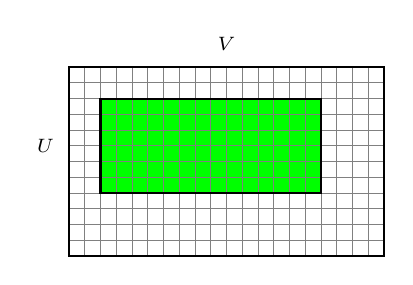
\begin{tikzpicture}
    \draw[fill = green] (0.4, -0.4) rectangle (3.2, -1.6);
    \draw[step = 0.2, gray, thin] (0, 0) grid (4, -2.4);
    \draw[black, thick] (0, 0) rectangle (4, -2.4);
    \draw[black, thick] (0.4, -0.4) rectangle (3.2, -1.6);
    \node at (-0.3, -1.) {\scriptsize $U$};
    \node at (2, 0.3) {\scriptsize $V$};
\end{tikzpicture}

            \end{center}
        \end{column}

		\begin{column}{0.48\textwidth}
            \begin{center}
                Треугольники:
                \vspace{0.2cm}
                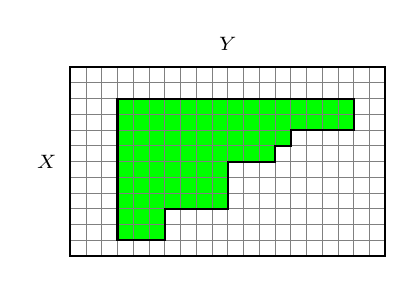
\begin{tikzpicture}
    \draw[fill = green] (0.6, -0.4) -- (3.6, -0.4) -- (3.6, -0.8) -- (2.8, -0.8) -- (2.8, -1) --
    	(2.6, -1) -- (2.6, -1.2) -- (2, -1.2) -- (2, -1.8) -- (1.2, -1.8) -- (1.2, -2.2) -- (0.6, -2.2) --
        cycle;
    \draw[step = 0.2, gray, thin] (0, 0) grid (4, -2.4);
    \draw[black, thick] (0.6, -0.4) -- (3.6, -0.4) -- (3.6, -0.8) -- (2.8, -0.8) -- (2.8, -1) --
    	(2.6, -1) -- (2.6, -1.2) -- (2, -1.2) -- (2, -1.8) -- (1.2, -1.8) -- (1.2, -2.2) -- (0.6, -2.2) --
        cycle;
    \draw[black, thick] (0, 0) rectangle (4, -2.4);
    \node at (-0.3, -1.2) {\scriptsize $X$};
    \node at (2, 0.3) {\scriptsize $Y$};
\end{tikzpicture}

            \end{center}
		\end{column}
	\end{columns}
\end{frame}



\begin{frame}{Иерархия}

    \tikzset{
    >=latex,
    perpinterface/.style = {
        postaction = {
            draw,
            decorate,
            decoration = {
                ticks,
                raise = 0.07cm,
                amplitude = 0.07cm,
                segment length = 1mm
            }
        }
    },
    % пружина
    vert/.style = {
        draw,
        ellipse
    },
    tikzart-fire/.pic = {
        \draw[fill = red!60] (0, 0) .. controls (0.3, 0) and (0.6, 0.1) .. (0.7, 0.3)
            .. controls (0.8, 0.5) and (0.85, 0.6) .. (0.8, 0.9)
            .. controls (0.75, 1.1) and (0.7, 1.2) .. (0.6, 1.4)
            .. controls (0.65, 1.2) and (0.6, 1.05) .. (0.5, 0.9)
            .. controls (0.5, 1.2) and (0.2, 1.3) .. (0.1, 1.6)
            .. controls (0.05, 1.75) and (0.1, 2) .. (0.2, 2.1)
            .. controls (-0.1, 2) and (-0.2, 1.85) .. (-0.3, 1.7)
            .. controls (-0.4, 1.5) and (-0.45, 1.3) .. (-0.4, 1.1)
            .. controls (-0.5, 1.2) and (-0.51, 1.4) .. (-0.5, 1.5)
            .. controls (-0.75, 1.2) and (-0.8, 0.7) .. (-0.7, 0.5)
            .. controls (-0.6, 0.28) and (-0.4, 0) .. (0, 0);
            \fill[white] (0, 0) .. controls (0.3, 0) and (0.52, 0.34) .. (0.37, 0.61)
            .. controls (0.4, 0.54) and (0.32, 0.32) .. (0.25, 0.25)
            .. controls (0.3, 0.35) and (0.25, 0.5) .. (0.2, 0.6)
            .. controls (0.1, 0.8) and (-0.05, 1) .. (0, 1.2)
            .. controls (-0.32, 1) and (-0.3, 0.72) .. (-0.2, 0.47)
            .. controls (-0.3, 0.51) and (-0.31, 0.6) .. (-0.33, 0.7)
            .. controls (-0.4, 0.6) and (-0.4, 0.5) .. (-0.4, 0.4)
            .. controls (-0.35, 0.18) and (-0.2, 0) .. (0, 0);
    }
}


    
\begin{tikzpicture}
    \node[vert] (res) at (1, 0) {$\Res$};
    \node[vert] (ns) at (-3, 0) {$\NS$};
    \node[vert] (cp) at (3, 1) {$\CP$};
    \node[vert] (acf) at (1.2, 1.5) {$\AC_0$-Frege};
    \node[vert] (resl) at (-1, 2.1) {$\ResL$};
    \node[vert] (acfp) at (0.5, 3.5) {$\AC_0[p]$-Frege};
    \node[vert] (fre) at (0.5, 5) {Frege};
    \node[vert] (ips) at (-2, 6) {$\PrSys{IPS}$};
    \node[vert] (pcr) at (-3, 2) {$\PCR[]$};
    \node[vert] (sos) at (-4, 2.5) {$\SOS$};

    \node[vert] (ns2) at (-5.5, 0) {$\NS_{\{\pm 1\}}$};
    \node[vert] (pcr2) at (-6, 2) {$\PCR[]_{\{\pm 1\}}$};
    \node[vert] (sos2) at (-6.8, 3) {$\SOS_{\{\pm 1\}}$};

    \node[vert] (cps) at (-4, 6.5) {$\PrSys{CPS}$};

    \draw[->] (res) -- (cp);
    \draw[->] (cp) to[out = 90, in = -20] (fre);
    \draw[->] (res) -- (resl);
    \draw[->] (res) -- (acf);
    \draw[->] (res) -- (pcr);
    \draw[->] (ns) -- (pcr);
    \draw[->] (resl) -- (acfp);
    \draw[->] (acf) -- (acfp);
    \draw[->] (acfp) -- (fre);
    \draw[->] (fre) -- (ips);
    \draw[->] (ips) -- (cps);

    \draw[->] (pcr) -- (ips);
    \draw[->] (sos) -- (cps);

    \draw[->] (ns2) -- (pcr2);
    \draw[->] (pcr2) -- (ips);
    \draw[->] (sos2) -- (cps);

    \node[inner sep = 0pt] at (-7, 5.5)
    {
\includegraphics[width = .2\textwidth]{pics/dragon.png}};

    \pause
    \draw[ultra thick, blue] (-4, -1) to[out = 110, in = 230] (-4.4, 3) to[out = 50, in = 180] (3.5, 1.8);
    \foreach \point in {(1.5, 3), (-2, 4), (-6, 1)}{
        \pic at \point {tikzart-fire};
    }
    
\end{tikzpicture}
    
\end{frame}
